\documentclass[10pt,pdf,hyperref={unicode}]{beamer}
\usepackage[utf8]{inputenc} 


\usepackage{lmodern}

% подключаем кириллицу 
\usepackage[T2A]{fontenc}
\usepackage[utf8]{inputenc}

\usepackage[utf8]{inputenc}
\usepackage[russian]{babel}
\usepackage{cmap}



\setbeamertemplate{caption}[numbered]

\usepackage{graphicx}
\graphicspath{{pictures/}}
\DeclareGraphicsExtensions{.pdf,.png,.jpg}


% отключить клавиши навигации
\setbeamertemplate{navigation symbols}{}

% тема оформления
\usetheme{boxes}

% цветовая схема
\usecolortheme{seahorse}

\title{Кто лучше <<Westeros Inc>> или <<Harpy \& Co>>?}   
\subtitle{Анализ качества стали}
\author{
Мареев Глеб, Меледин Станислав, Сударева Валерия, Шуган Алёна} 
\date{20 апреля 2018 года} 




\begin{document}

% титульный слайд
\begin{frame}
\titlepage
\end{frame} 

\begin{frame}
\frametitle{Метод} 
\framesubtitle{}
Для составления рекомендаций: какого поставщика стали выбрать для заключения эксклюзивного контракта, необходимо найти сильные стороны каждого поставщика. 

Сделаем это посчитав различные статистики и построив их графики для каждой компании.

После этого поймем: какого поставщика в каком случае нужно выбирать.
\end{frame}


\begin{frame}
\frametitle{Общее количество произведенных и поломанных мечей} 
\framesubtitle{}

\begin{minipage}{0.4\textwidth}
 	\begin{figure}[L]
		\center{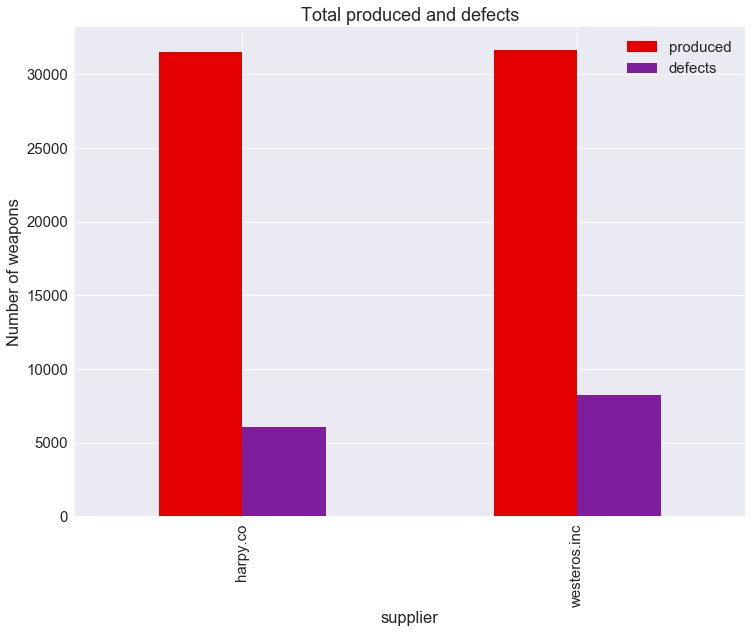
\includegraphics[width=180px]{1.png}}
		\caption{Общее количество произведенных и поломанных мечей}	
	\end{figure}
\end{minipage}
\hfill
\begin{minipage}{0.4\textwidth}
	У <<Westeros Inc>> объем произведенных мечей не намного больше, но количество поломанных мечей сильно превосходит компанию <<Harpy & Co>>.   
\end{minipage}
\end{frame}

\begin{frame}
\frametitle{Отношение числа сломанных мечей к произведенным} 
\framesubtitle{}

\begin{minipage}{0.4\textwidth}
 	\begin{figure}[L]
		\center{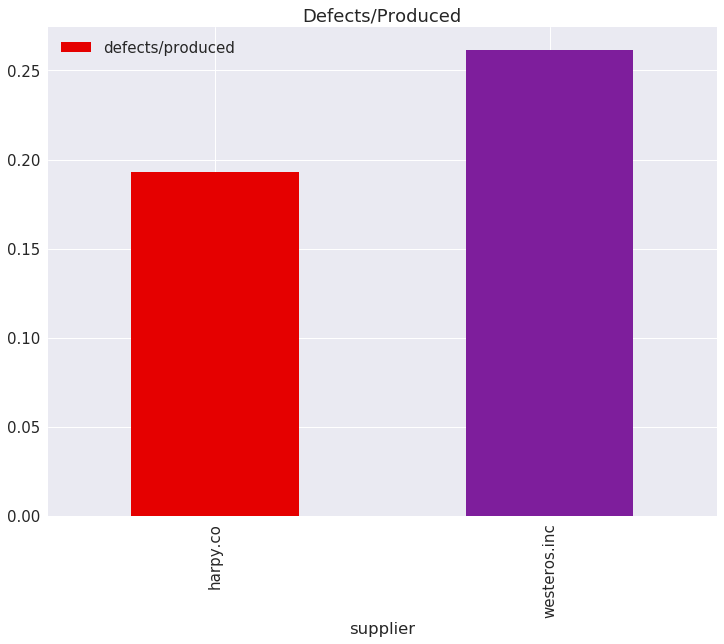
\includegraphics[width=180px]{2.png}}
		\caption{Отношение числа сломанных мечей к произведенным}		
	\end{figure}
\end{minipage}
\hfill
\begin{minipage}{0.4\textwidth}
	У компании <<Westeros Inc>> больший процент отношения $\frac{\text{Кол-во сломанных мечей}}{\text{Кол-во произведенных мечей}}$. 
\end{minipage}
\end{frame}


\begin{frame}
\frametitle{Тенденция к поломке мечей с течением времени (в среднем)} 
\begin{minipage}{0.4\textwidth}
 	\begin{figure}[L]
		\center{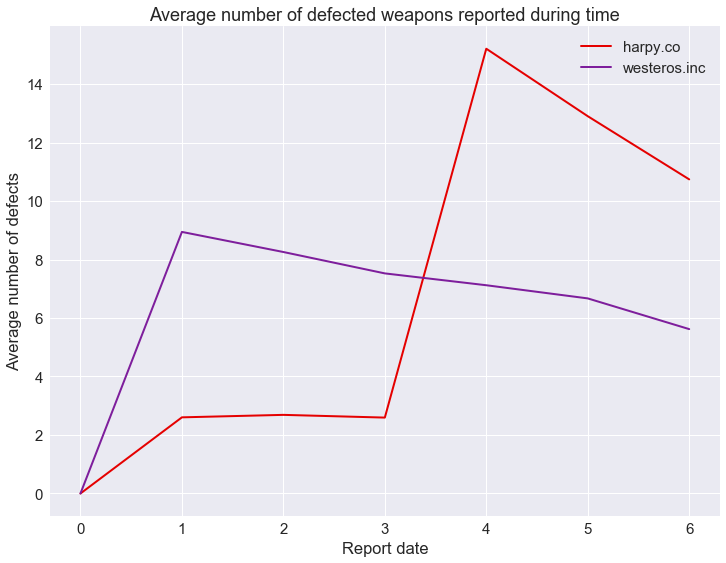
\includegraphics[width=180px]{3.png}}
		\caption{Среднее количество сломанных мечей с течением времени}
	\end{figure}
\end{minipage}
\hfill
\begin{minipage}{0.4\textwidth}
	У компании <<Westeros Inc>> мечи в среднем ломаются быстрее - уже на второй месяц среднее количество поломанных мечей у <<Westeros Inc>> больше примерно в 4 раза. 
	Однако после 3 месяца службы мечи <<Harper Co>> начинают активно ломаться и стремительно обгоняют конкурентов по среднему количеству дефектов. 
\end{minipage}
\end{frame}

\begin{frame}
\frametitle{Тенденция к поломке мечей с течением времени (по итоговым данным)} 
\framesubtitle{}

\begin{minipage}{0.4\textwidth}
 	\begin{figure}[L]
		\center{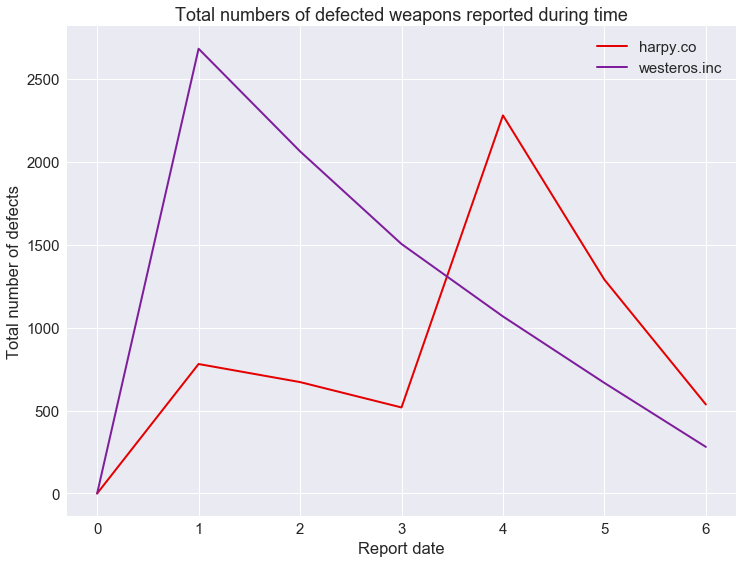
\includegraphics[width=180px]{4.png}}
		\caption{Общее количество сломанных мечей с течением времени}	
	\end{figure}
\end{minipage}
\hfill
\begin{minipage}{0.4\textwidth}
	По общему количеству сломанной продукции в первые несколько месяцев <<Westeros Inc>> значительно превосходит конкурента. 
	И даже несмотря на то, что после третьего месяца оружие <<Harper Co>> имеет свойство изнашиваться и ломаться, "пик" графика дефектов <<Harper Co>> все равно находится ниже "пика" аналогичного графика у <<Westeros Inc>>. Хотя в целом, начиная с третьего месяца, количество сломанных мечей у <<Harper Co>> больше.    
\end{minipage}
\end{frame}


\begin{frame}
\frametitle{Среднее количество дефектов во время производства} 
\framesubtitle{}

\begin{minipage}{0.4\textwidth}
 	\begin{figure}[L]
		\center{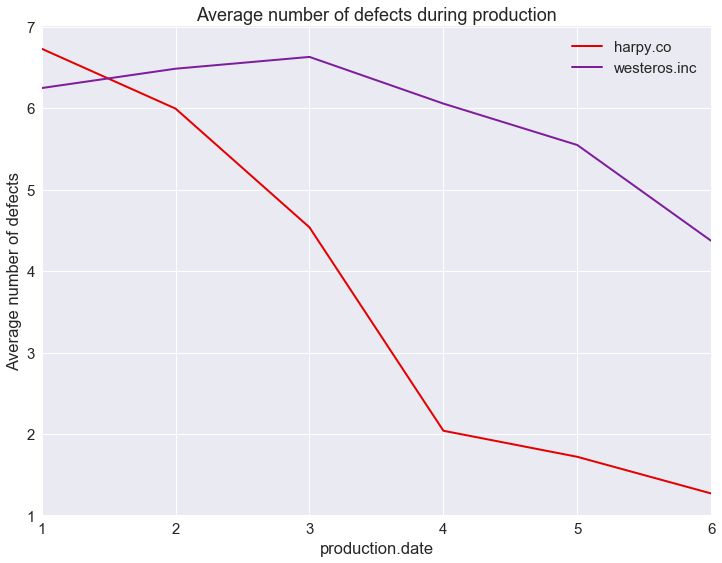
\includegraphics[width=180px]{5.png}}
		\caption{Среднее количество дефектов во время производства}	
	\end{figure}
\end{minipage}
\hfill
\begin{minipage}{0.4\textwidth}
	Среднее количество поломанных мечей стремительно идет вниз у компании <<Harpy Co>> в течение 6 месяцев, в то время как у компании <<Westeros Inc>> это значение лишь незначительно уменьшается. Итого количество поломок больше у <<Westeros Inc>>. 
\end{minipage}
\end{frame}


\begin{frame}
\frametitle{Итоговое количество дефектов в течение всего производства} 
\framesubtitle{}

\begin{minipage}{0.4\textwidth}
 	\begin{figure}[L]
		\center{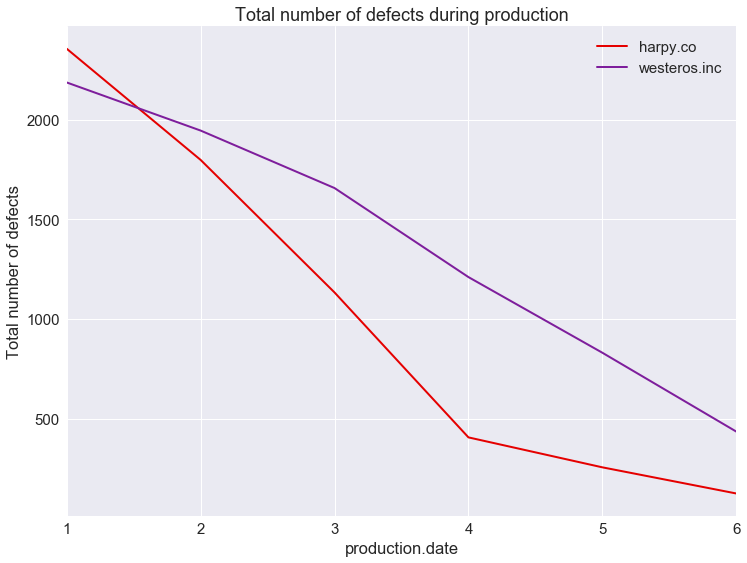
\includegraphics[width=180px]{6.png}}
		\caption{Итоговое количество дефектов во время производства}	
	\end{figure}
\end{minipage}
\hfill
\begin{minipage}{0.4\textwidth}
	Итоговое количество сломанных мечей в месяц уменьшается в течение времени производства у обоих компаний. Тем не менее, у <<Harpy Co>> эта тенденция более выражена, и итоговое количество поломанных мечей меньше в течение всего времени.  
\end{minipage}
\end{frame}


\begin{frame}
\frametitle{Итоговое количество дефектов (относительно кузнецов)} 
\framesubtitle{}

\begin{minipage}{0.4\textwidth}
 	\begin{figure}[L]
		\center{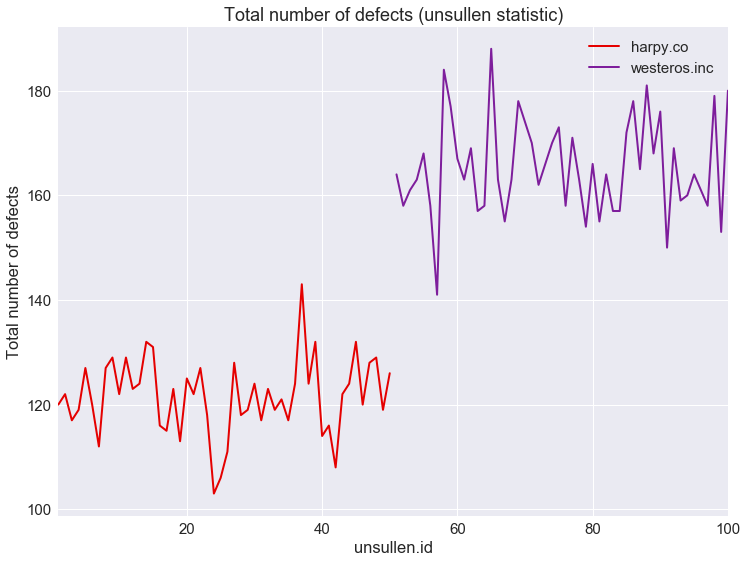
\includegraphics[width=180px]{7.png}}
		\caption{Итоговое количество сломанных мечей}	
	\end{figure}
\end{minipage}
\hfill
\begin{minipage}{0.4\textwidth}
	У обоих компаний среднее отклонение от общего количества поломок для каждого из кузнецов приблизительно одинаковое. На этом же графике видно что в общем и целом у <<Westeros Inc>> на каждого кузнеца приходится больше поломок, чем у <<Harpy Co>>.   
\end{minipage}
\end{frame}


\begin{frame}
\frametitle{Общий объем производства} 
\framesubtitle{}

\begin{minipage}{0.4\textwidth}
 	\begin{figure}[L]
		\center{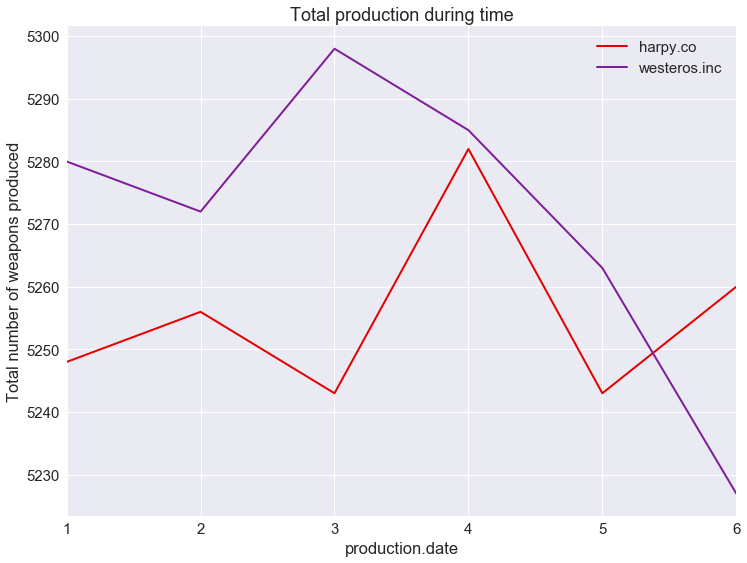
\includegraphics[width=180px]{8.png}}
		\caption{Общее количество произведенного оружия}	
	\end{figure}
\end{minipage}
\hfill
\begin{minipage}{0.4\textwidth}
	Можно заметить, что объем производства у <<Westeros Inc>> на протяжении 90 процентов времени выше, чем у <<Harpy Co>>. Тем не менее, под конец времени производства количество выпущенного товара у <<Westeros Inc>> стремительно падает, что значительно портит общую статистику, так, что итоговое количество произведенных мечей у обоих компаний лишь незначительно отличается.  
\end{minipage}
\end{frame}


\begin{frame}
\frametitle{Общее производство (относительно кузнецов)} 
\framesubtitle{}

\begin{minipage}{0.4\textwidth}
 	\begin{figure}[L]
		\center{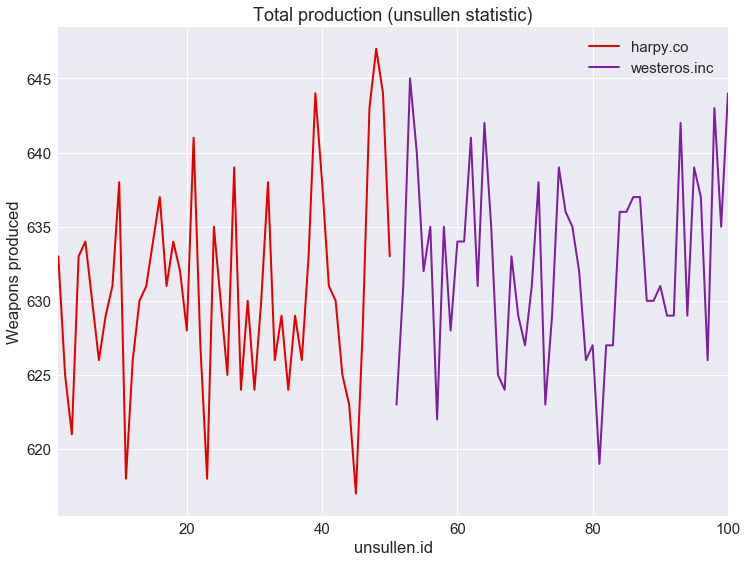
\includegraphics[width=180px]{9.png}}
		\caption{Общее количество произведенного оружия}	
	\end{figure}
\end{minipage}
\hfill
\begin{minipage}{0.4\textwidth}
	По графику можно сделать вывод, что эффективность работы кузнецов у обоих компаний примерно на одном уровне, но у <<Harpy Co>> разброс больше - некоторые кузнецы работают очень хорошо, некоторые - откровенно плохо. У <<Westeros Inc>> такого сильного разброса не наблюдается.   
\end{minipage}
\end{frame}

\begin{frame}
\frametitle{Итоговое количество НЕсломанных мечей (относительно кузнецов)} 
\framesubtitle{}

\begin{minipage}{0.4\textwidth}
 	\begin{figure}[L]
		\center{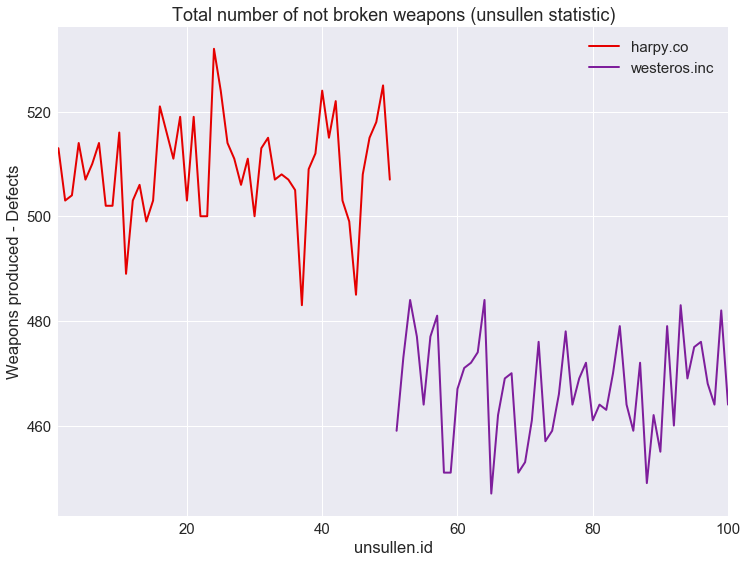
\includegraphics[width=180px]{10.png}}
		\caption{Количество не сломанного оружия (статистика относительно кузнецов)}	
	\end{figure}
\end{minipage}
\hfill
\begin{minipage}{0.4\textwidth}
	В целом кузнецы в <<Harpy Co>> делают более надежные мечи.
\end{minipage}
\end{frame}



\begin{frame}
\frametitle{Тенденция к производству более надежных мечей} 
\framesubtitle{}

\begin{minipage}{0.4\textwidth}
 	\begin{figure}[L]
		\center{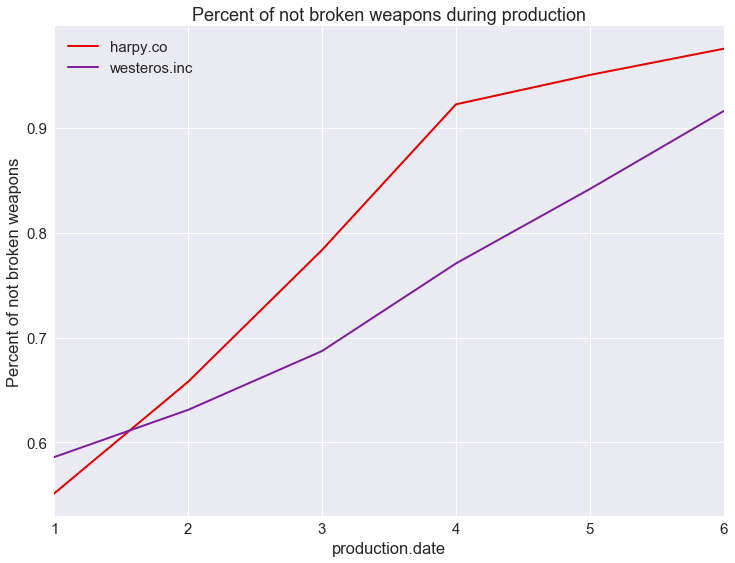
\includegraphics[width=180px]{11.png}}
		\caption{Процент несломанных мечей с течением времени}		
	\end{figure}
\end{minipage}
\hfill
\begin{minipage}{0.4\textwidth}
	Во время производства у компании <<Harpy \& Co>> тенденция к производству более прочных мечей выражена сильнее, чем у <<Westeros Inc>>, и общая надежность оружия выше. 
\end{minipage}
\end{frame}


\begin{frame}
\frametitle{Общее количество несломанных мечей} 
\framesubtitle{}

\begin{minipage}{0.4\textwidth}
 	\begin{figure}[L]
		\center{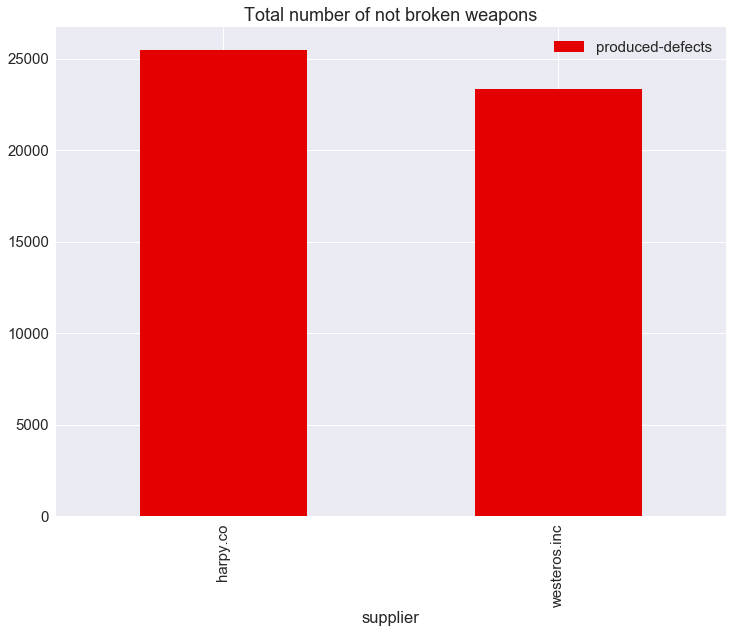
\includegraphics[width=180px]{12.png}}
		\caption{Общее число несломанных мечей}	
	\end{figure}
\end{minipage}
\hfill
\begin{minipage}{0.4\textwidth}
	По итоговому объему несломанных мечей, изготовленных из стали, лидирует компания <<Harpy.co>>. 
\end{minipage}
\end{frame}



\begin{frame}
\frametitle{Выводы} 

В итоге пришли к следующим выводам:
\begin{itemize}
\item Если необходим большой объем выпуска, но при этом не так важно качество мечей - можно выбрать <<Westeros Inc>>.
\item Мы рекомендуем компанию <<Harpy \& Co>>, так как их мечи в целом надежнее, хотя и имеют свойство изнашиваться и ломаться после нескольких месяцев службы. Мастерство кузнецов <<Harpy Co>> превосходит конкурентов и со временем прогрессирует в значительной степени, и с каждым новым выпуском мечи становится более прочными. 
\end{itemize}
\end{frame}

\end{document}